\chapter{Materials and Method}
\label{cha:materials_and_method}

\section{Dataset}
\label{sec:dataset}

\subsection{Generation}
\label{subsec:generation}

We created our dataset from approximately $3,000$ scientific articles in PDF format. An important point was that these articles come from different scientific fields.

We used a text mining pre-processing technique as introduced by Vijayarani et al.~\cite{Vijayarani2015} to separate the text from the PDFs and add additional information. This technique consists of three key steps, which are called extraction, stopword removal, and stemming. First, we used a framework described in ~\cite{KlampflGJK14} to separated the article structure and the raw text from the PDF. Afterwards the stopwords are removed, and the remaining terms of the raw text are stemmed.

\begin{table}[!b]
  \centering
  \begin{tabular}{C{2.6cm} C{2.7cm} C{1.5cm} C{1.5cm} C{1.5cm} C{1.5cm}}
    \toprule
    & \multicolumn{3}{c}{\textbf{per Section}} & \multicolumn{2}{c}{\textbf{Overall}} \\
    \textbf{IMRaD Type} & \textbf{Section Title} & \textbf{\# Paper} & \textbf{Percent} & \textbf{\# Paper} & \textbf{Percent} \\ \midrule
    Introduction & Introduction & $822$ & $100\%$ & $822$ & $100\%$ \\ \midrule
    Background & Related Work & $465$ & $56.57\%$ & $465$ & $56.57\%$ \\ \midrule
    \multirow{3}{*}{Methods} & Method & $97$ & $11.8\%$ & \multirow{3}{*}{$312$} & \multirow{3}{*}{$37.96\%$} \\
    & Model & 134 & $16.3\%$ \\
    & Approach & 81 & $9.85\%$ \\ \midrule
    \multirow{3}{*}{Result} & Experience & $396$ & $48.18\%$ & \multirow{3}{*}{$687$} & \multirow{3}{*}{$83.58\%$} \\
    & Result & 163 & $19.83\%$ \\
    & Evaluation & 128 & $15.57\%$ \\ \midrule
    \multirow{3}{*}{Discussion} & Conclusion & $581$ & $70.68\%$ & \multirow{3}{*}{$773$} & \multirow{3}{*}{$94.04\%$} \\
    & Discussion & 179 & $21.78\%$ \\
    & Future Work & 13 & $1.58\%$ \\
    \bottomrule
  \end{tabular}
  \caption[Mapping of the Section Titles to IMRaD-Types]{\textbf{Mapping of the Section Titles to IMRaD-Types.} In this Table we show which section titles was used to generate the IMRaD structure information. Additionally, we show the relation between titles and how often they occurs in the used dataset.}
  \label{tbl:mapping_section_names}
\end{table}

One additional information we had to add was IMRaD structure (see \Cref{sec:imrad_structure}). The IMRaD structure maps \textit{Related Work} to be part of the \textit{Introduction}. Since most of our papers had an own section titled \textit{Related Work} we introduce an additional type called \textit{Background} for it. We were able to classify the IMRaD structure with simple keyword detection in the section titles. \Cref{tbl:mapping_section_names} shows the mapping between IMRaD-Types and these titles. Because it was not really possible to identify \textit{Method} sections by using the section titles we used information about their position in the article. We manage that by using the \textit{Background} section as upper bound, and the \textit{Result} section as lower bound. We classify all sections between these two bounds as a \textit{Method} section. When the \textit{Background} section was not available, we set the \textit{Introduction} section as upper bound. Additionally, when the \textit{Result} section was not available, we set the \textit{Discussion} section as lower bound. If one of the two bounds could not be set, we discarded the scientific article. Note that, chapters can have several IMRaD-Types. For example, if a section was titled \textit{"Results and Discussion"} it belongs to the types \textit{Result} and \textit{Discussion}.

Another additional detail we had to add were links between the scientific articles. For this we performed a semi-automated annotation. Thereby similarities about the references of an article and the titles of all other articles are compared, and if they exceed a given threshold a recommendation to create a link between the two was given.

We created each data record in such a way that it can be transferred directly to the database schema shown in \Cref{fig:database_schema}. To reduce noise during the evaluation we removed all articles without any connection to other articles.

Finally, we have $821$ scientific articles in our dataset. This are only $27$ percent of the initial set. This small number is due to the environment and the used scientific articles. One major problem was that the framework used to separate the structure had issues with documents that were not created with latex.

\myfig{database_schema}
      {width=0.70\textwidth}
      {Database Schema for the used Dataset}
      {Database Schema for the used Dataset}
      {fig:database_schema}

\subsection{Structure of a Scientific Article}
\label{sec:structure_scientific_article}

We designed a database schema, which corresponds to the structure of a scientific article. The table "scientific article" in the schema (see \Cref{fig:database_schema}) can be seen as the root node for each database entry.

The "author text" attribute refers to the table "AuthorText". It contains the names and email addresses of all associated authors. These values are generated from the author area, which is normally on the first page of each paper. In the database schema this attribute consists of three values. First, the complete text, which contains the whole author area. Second, the email text, which are all email addresses separated from the complete text. Finally, a list with all authors. The author area is the only area that is not prepossessed.

\myfig{scientific_articles_tree}
      {width=0.90\textwidth}
      {\textbf{Example of a Scientific Article Tree.} In this figure we highlight the hierarchical structure of an typical scientific article. For example it can be composed into multiple sections.}
      {Example of a Scientific Article Tree.}
      {fig:scientific_articles_tree}

One of the most important characteristics are sections, and the underlying structure. \Cref{fig:scientific_articles_tree} shows an example of an article, and the tree-like structure that comes with it. Chapters are non-leaf nodes, and text areas are leaf nodes. This is represented in database schema as two lists, one for subsections and one for text areas. In addition to the lists, each section itself has a section type. This attribute describes whether the section is a section, subsection, or subsubsection. The IMRaD structure information is stored as the IMRaD-Type. As described in \Cref{subsec:generation}, each section may have several IMRaD-Types. Each type of section holds its own list of these types. Hence, subsections and subsubsections keep the same IMRaD-Types as their parent section.

We store word histograms for articles as well as the sections, so we do not have to scan the entire text for each search request. These histograms contain the term frequencies of the corresponding area. Therefore, subsubsections contain the frequencies of their text areas, subsections contain the frequencies of their text areas, and their subsubsections text areas, and so on. Finally, an article holds the term frequencies of the whole document.

The last two attributes of an article are the reference-, and the cited-by-lists. The two lists are used to generate connections between articles. A reference holds the identifier of a referred paper. In turn, the referred paper has an entry with the paper id in the cited-by-list. Additionally, we store the text of whole reference, the authors, and other available information such as publisher, pages, or the volume.

One characteristic over all tables of the schema is, that all extracted text values are available as raw-, and processed text values. Raw represents the text as it was separated from the used framework. Processed is the raw text after the stopword removal and the stemming.

\subsection{Citation Network}
\label{sec:citation_network}

\myfig{dataset_generall}
      {width=0.50\textwidth}
      {\textbf{General Structure of a Citation Network.} The timeline indicates that new articles citing existing articles, and thus there can not be cyclic dependencies between them.}
      {General Structure of a Citation Network}
      {fig:structure_citation_network}

A Citation network represents the relationship between scientific articles. In general citation means that one article mentions the work of another article. Therefore a
reference with the title, the authors and the publication journal is added. \Cref{fig:structure_citation_network} shows the structure of such a network. Scientific articles are nodes, and citations are directed edges between these nodes. The timeline indicates that new articles are citing already existing articles, and thus there can not be cyclic dependencies.

M. Kas ~\cite{kas2011} defined the basic properties of citation networks in their work. In our case the most important ones are:

\begin{itemize}
  \item Directed.
  \item Acyclic.
  \item All edges point backwards in time
  \item Edges are permanent
  \item The existing part is mostly constant. Only the leading edges changes
\end{itemize}

The network is directed and acyclic because each article has a publication date and can only cite previously published articles. Due to these properties edges can only point back in time. The edges of the network have to be permanent because the references of the existing articles never change. When a new node is added it generates edges to existing articles. This means that all other nodes and edges stays constant.

\begin{table}[!b]
  \centering
  \begin{tabular}{ l c }
    \toprule
    \textbf{Number of Nodes}      & $821$  \\ \midrule
    \textbf{Number of Edges}      & $1,716$ \\ \midrule
    \textbf{Longest Path Length}  & $12$   \\ \midrule
    \textbf{Number of Root Nodes} & $107$  \\
    \bottomrule
  \end{tabular}
  \caption[General Properties about the citation network]{\textbf{General Properties about the citation network.} The citation network represents the relationship between our used scientific articles. The number of nodes indicates the number of articles, and the number of edges citations between those articles. There are no cycles inside the graph, and the longest citation chain consists of $12$ articles. There are $107$ articles which has no outgoing edges. That means that none of their referred articles are part of our dataset.}
  \label{tbl:general_properties_about_the_graph}
\end{table}

The main properties of our citation network are shown in \Cref{tbl:general_properties_about_the_graph}. Scientific articles are the nodes, and citations are the edges between these nodes. This means that our network consists of $821$ articles, and $1,716$ citations between these articles. During the generation of our dataset we found cycles due to preprints. Preprints are versions of scientific articles which are not peer reviewed, and published in a scientific journal. In our case we removed all preprints from the dataset. The longest path length indicates that the longest citation chain of our network consists of $12$ articles. The root nodes are nodes without any outgoing edges. In our network are $107$ root articles which cite no other article. This happens because none of their referred articles are part of our dataset.

\begin{figure}[!t]
  \begin{minipage}{\textwidth}
    \begin{minipage}[b]{0.39\textwidth}
      \centering
      \begin{tabular}{ l c }
        \toprule
        \textbf{Max References}    & $98$     \\ \midrule
        \textbf{Mean References}   & $5.8767$ \\ \midrule
        \textbf{Median References} & $2$      \\
        \bottomrule
    \end{tabular} \\
    \vspace*{1cm}
    (a) Properties
  \end{minipage}
  \begin{minipage}[b]{0.59\textwidth}
    \centering
    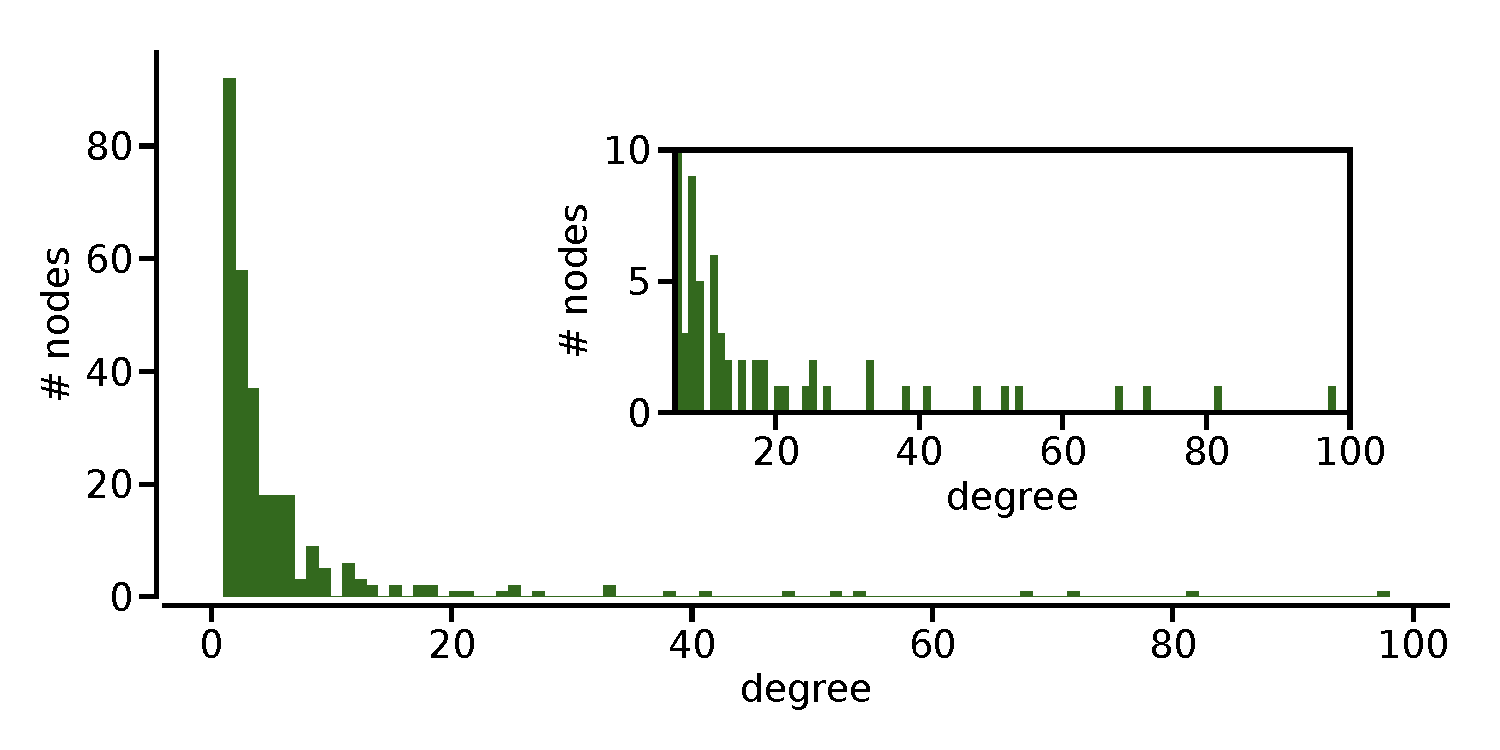
\includegraphics[width=1.0\textwidth]{figures/in-degree_distribution} \\
    (b) In-Degree Distribution
    \end{minipage}
  \end{minipage}
  \caption[In-Degree Distribution of the Citation Network]{\textbf{In-Degree Distribution.} The in-degree distribution describes how often articles get referred by other articles. The long tail of the distribution indicates that there are a lot of articles which are cited only a few times, and a few articles which are cited more often. There are some outliers with a higher degree than $20$. This can also be seen by the difference between the mean and the median. The maximum number of references in connection with the zoomed view represents that one single article was cited by $98$ other articles.}
  \label{fig:indegree_distribution}
\end{figure}

\Cref{fig:indegree_distribution} describes the in-degree distribution of our citation network. In general, the in-degree of a node is the number of ingoing edges. The in-degree distribution represents the probability distribution of these nodes over the whole network. Regarding a citation network the in-degree of a node is the number of articles which referred to this article. The long tail of the in-degree distribution indicates that there are a lot of articles which are referred only a few times, and a few articles which are referred more often. There are only some articles with an in-degree higher than $20$. The maximum number of references in connection with the zoomed view represents that one single article was referred by $98$ other articles.

\begin{figure}[!t]
  \begin{minipage}[!t]{\textwidth}
    \begin{minipage}[b]{0.39\textwidth}
      \centering
      \begin{tabular}{ l c }
        \toprule
        \textbf{Max References}    & $13$     \\ \midrule
        \textbf{Mean References}   & $2.4034$ \\ \midrule
        \textbf{Median References} & $2$      \\
        \bottomrule
    \end{tabular} \\
    \vspace*{1cm}
    (a) Properties
  \end{minipage}
  \begin{minipage}[b]{0.59\textwidth}
    \centering
    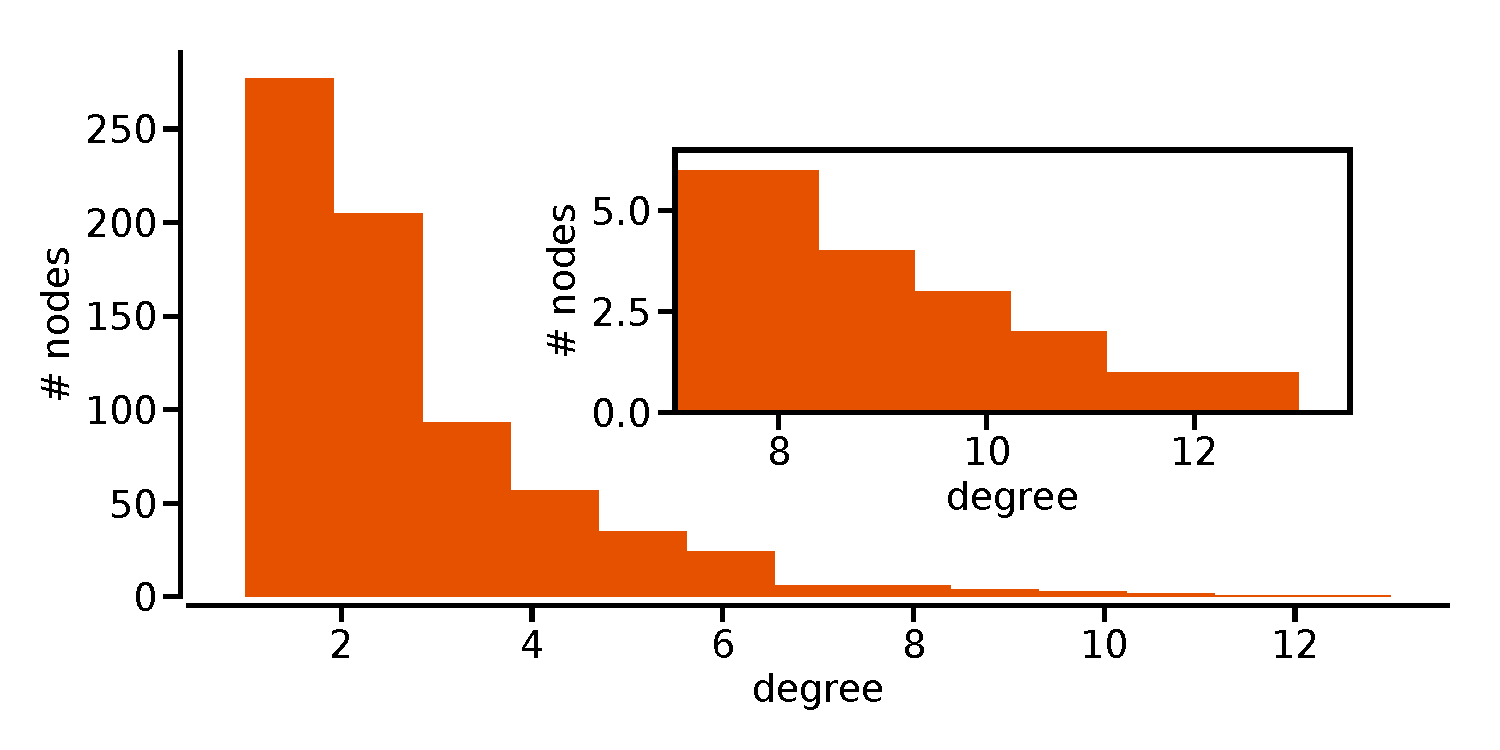
\includegraphics[width=1.0\textwidth]{figures/out-degree_distribution} \\
    (b) Out-Degree Distribution
    \end{minipage}
  \end{minipage}
\caption[Out-Degree Distribution of the Citation Network]{\textbf{Out-Degree Distribution.} The out-degree distribution describes how often articles refer other articles. The long tail of the distribution indicates that there are a lot of articles which refer less than $7$ other articles, and only few with refer to more articles. Mean and median of the outgoing edges are low, because not every refereed article is part of our dataset. By the small difference between the mean and the median can be seen that there are less outliers. The maximum number of references represent that the highest number of a single article refers other articles is $13$.}
\label{fig:outdegree_distribution}
\end{figure}

The out-degree distribution and their properties are displayed in \Cref{fig:outdegree_distribution}. In contrast to the in-degree distribution, the out-degree distribution describes the number of outgoing edges. Regarding to the citation network, the out-degree of a node can be described as the number of articles which gets referred by this article. The long tail of the out-degree distribution indicates that there are a lot of articles which refer less than $7$ other articles, and only few with refer $7$ or more articles. Mean and median of the outgoing edges are low, because not every refereed article is part of our dataset. By the small difference between mean and median we can also see that there are less outliers. The maximum number of references represent the highest number of a single article refers to other articles, which is in our case $13$.

\section{Model}
\label{sec:model}

An information retrieval model is defined by the quadruple $[\textbf{D}, \textbf{Q}, \mathcal{F}, \mathcal{R}(q_i, d_j)]$ that contains the design of documents in the document collection $\textbf{D}$, queries $\textbf{Q}$, the framework $\mathcal{F}$, and the ranking function $\mathcal{R}(q_i, d_j)$ (cf. \Cref{sec:information_retrieval_models}). We design our system with the goal to compare various common ranking algorithms. Therefore, we generate a model that allows that ranking algorithms can easily be exchanged by a configuration parameter. Additionally, our model is designed to work with unstructured as well as structured data. This is reflected by the query language. 

For structured text retrieval, we structure the documents according to their IMRaD sections (see \Cref{sec:imrad_structure}). In our dataset the background chapter is available in addition to the IMRaD chapters. Therefore, it was introduced as an additional IMRaD type.

We define documents to provide data unstructured and structured. Hence, each document in the dataset contains a bag of words where all index terms of its text content ($DBW_{\textit{All}}$) are stored. In a bag of words each term is represented as a pair of term and term frequency. Additionally, the documents contain $5$ bag of words for each IMRaD-type ($DBW_\textit{Introduction}$, $DBW_\textit{Background}$, $DBW_\textit{Methods}$, $DBW_\textit{Results}$, $DBW_\textit{Discussion}$), where: 
\begin{align}
  DBW_\textit{IMRaD} = &DBW_\textit{Introduction} \cup DBW_\textit{Background} \cup DBW_\textit{Methods} \nonumber \\
                       &\cup DBW_\textit{Results} \cup DBW_\textit{Discussion}.
\end{align}
$DBW_\textit{IMRaD}$ differs from $DBW_{\textit{All}}$, as there exist areas in the document that cannot be assigned to an IMRaD-type (e.g., Abstract).

%\lstset{language=XML}
%\begin{lstlisting}
%<document>
%  <h1>Introduction</h1>
%  <p>I love deadlines.</p>
%  <h1>Methods</h1>
%  <p>I like the whooshing sound they make as they fly 
%     by.</p>
%</document>
%\end{lstlisting}

We remove stopwords and stem words during the indexing process of a document to generate index terms. Afterwards, we assign the index terms to bag of words of a document. For example, "\textit{I love deadlines.}" is in the \textit{Introduction} and "\textit{I like the whooshing sound they make as they fly by.}" is in the \textit{Methods} of a document $A$. The underlying bags of words in the document are given by:
\begin{equation}
  \label{bag_of_words_example_A}
  \begin{split}
  DBW_{\textit{All}} &= \{"\textit{love}": 1, "\textit{deadlin}" : 1, "\textit{whoosh}" : 1, "\textit{sound}": 1, "\textit{fly}": 1\} \\ 
  DBW_{\textit{Introduction}} &= \{"\textit{love}": 1, "\textit{deadlin}": 1\} \\
  DBW_{\textit{Methods}} &= \{"\textit{whoosh}": 1, "\textit{sound}": 1, "\textit{fly}": 1\}.
  \end{split}
\end{equation}
We represent IMRaD sections that do not occur in the document by an empty bag of words. In this example, the union of $DBW_{\textit{Introduction}}$ and $DBW_{\textit{Methods}}$ is similar to $DBW_{\textit{All}}$. When we define $A$ to additionally contain "\textit{I love music.}" in the \textit{Abstract} then $DBW_{\textit{All}}$ changes, but $DBW_{\textit{Introduction}}$ and $DBW_{\textit{Methods}}$ stay the same.

We define the query language in a way that the user can choose if unstructured or structured text retrieval is used. Therefore, we design an IN-statement that connects query terms and IMRaD-Types. For example, with the query "\textit{local}, \textit{network} IN \texttt{Methods}" a user can specify that the terms \textit{local} and \textit{network} should occur in the \texttt{Methods} section of a document. 

The left part of the IN-statement is converted into a set of query terms. Hence, multiple occurrences of a single term in the query does not affect the outcome. The right part of the IN-statement captures in which set the query term is stored. Therefore, given the $5$ IMRaD-Types we defined $6$ query sets ($QS_{\textit{All}}$, $QS_{\textit{Introduction}}$, $QS_{\textit{Background}}$, $QS_{\textit{Methods}}$, $QS_{\textit{Results}}$, $QS_{\textit{Discussion}}$). The query sets are connected directly to the documents bags of words in the framework. For example, the terms in $QS_{\textit{Introduction}}$ are used to search in $DBW_{\textit{Introduction}}$.

When a query contains terms without any IN-statements the terms are added to $QS_{\textit{All}}$. Hence, query terms are stored in an IMRaD query set if an IN-statement is present, or in $QS_{\textit{All}}$ otherwise. As a result, query terms are searched in $DBW_{\textit{All}}$ or $DBW_\textit{IMRaD}$, but never in both of them. This query structure avoids the usage of unstructured and structured text retrieval with a single request.

We introduce an AND-statement to combine multiple IN-statements. For example, "\textit{area} IN \texttt{Background}" AND "\textit{local}, \textit{network} IN \texttt{Methods}" expresses that \textit{area} should occur in \texttt{Background} section and the terms \textit{local} and \textit{network} should occur in the \texttt{Methods} section of a document. Therefore, "\textit{area}" is added to $QS_{\textit{Background}}$ and "\textit{local}", "\textit{network}" is added to $QS_{\textit{Methods}}$. The definition of the AND-statement allows to search multiple bags of words with a single request. We combine the query sets on the left part of the IN-statement at query time when an IMRaD type appears multiple times. The same holds when unstructured text retrieval is used (e.g., "\textit{area}" AND "\textit{local}, \textit{network}").

Only one query term has to occur in the specified bag of words to mark a document as relevant. This increases the number of relevant documents in the resulting ranked list. For example, a query is given by "\textit{plane} IN \texttt{Introduction}" AND "\textit{fly} IN \texttt{Methods}". When document $A$ in the previous example (see \Cref{bag_of_words_example_A}) is searched with respect to the defined query it will be marked as relevant. This happens as \textit{fly} appears in $DBW_{\textit{Methods}}$. We design our system that the maximum number of relevant documents in a generated ranked list can be set via a configuration parameter. Per default this setting is disabled.

In our system, it is possible to use entire documents (in PDF format) to search for other documents. In this case, the user has to specify if unstructured or structured text retrieval should be used. The specification influences the generation of the query sets $QS$. The system processes query sets generated by a document the same way as they are generated by a query. To transform a document into query sets we perform the following steps: 
\begin{enumerate}
 \item First, we extract the article structure and the text content from the PDF. To that end, we use a framework described in ~\cite{KlampflGJK14}.
 \item Second, we map section headings to IMRaD sections by keyword detection. We apply a similar approach to map the \textit{Methods} section as we did for the generation of the dataset (see \Cref{subsec:generation}). The only difference is that a document will not be rejected if the upper or lower bound cannot be detected. In that case, the \textit{Methods} section is not mapped. This step is only performed for structured text retrieval, as IMRaD-Type detection is not necessary for unstructured text retrieval.
 \item Third, we remove stopwords and stem terms for the whole content of the document.
 \item The fourth step differs depending on the usage of unstructured or structured text retrieval: 
 \begin{itemize}
  \item For unstructured text retrieval, we added all terms to $QS_{\textit{All}}$.
  \item For structured text retrieval, we added the terms to a query set with respect to the IMRaD-Type of the section they occur.
 \end{itemize}
\end{enumerate}
Finally, our system searches for other documents with the usage of the generated query sets. Therefore, we calculate a rank for each document that contains query words in the specified section. In \Cref{sec:unstructured_text_Retrieval} we discuss several ranking algorithms. All of them calculate rankings based on a query $q$, and a document $d_j$. For unstructured text retrieval, the ranking algorithms are used without any transformation as $QS_{\textit{All}}$ represents the query and $DBW_{\textit{All}}$ the document.

We change the calculation of the rank for structured text retrieval to take the IMRaD structure into account: 
\begin{align}
  \label{imrad_formula}
  sim(d_j, q) = \frac{1}{|\text{IMRaD-TYPES}|} \times \sum_{k \in \text{IMRaD-TYPES}} sim(d_{j, k}, q_k), 
\end{align}
where IMRaD-TYPES is an array containing all IMRaD-Types. The document $d_j$ is a dictionary that contains all IMRaD bags of words, and $d_{j, k}$ is the bag of words of IMRaD-type $k$. Furthermore, $q$ is a dictionary containing all query sets, and $q_k$ is the query set of IMRaD-type $k$. However, for structured text retrieval the mean rank over all IMRaD-types is assigned to be the documents rank.

In our system, \textit{Term Frequency (TF)}, \textit{Term Frequency - Inverse Document Frequency (TF-IDF)}, \textit{BM$25$}, \textit{Divergence from Randomness (DfR)}, and \textit{Ranked Boolean Retrieval (RBR)} are available as ranking algorithms. A configuration parameter defines which ranking algorithm is used. Additional parameters of the ranking algorithm (e.g., $b$ and $K_1$ for BM$25$) are also added to the configuration. 

The simplest ranking algorithm is \textit{TF}. It sums the frequencies given in a bag of words, for all terms in a query set. For example, document $B$ is given by:
\begin{equation}
  \label{bag_of_words_example_B}
  \begin{split}
  DBW_{\textit{All}} &= \{"\textit{love}": 5, "\textit{deadlin}" : 1, "\textit{whoosh}" : 2 \} \\ 
  DBW_{\textit{Introduction}} &= \{"\textit{love}": 3, "\textit{deadlin}": 1\} \\
  DBW_{\textit{Methods}} &= \{"\textit{love}": 2, "\textit{whoosh}": 2 \}.
  \end{split}
\end{equation}
Furthermore, we configure \textit{TF} as ranking algorithm and a query is given by "\textit{love}, \textit{whoosh}". Hence, $QS_{\textit{All}} = \{"\textit{love}", "\textit{whoosh}"\}$ and the rank of $B$ is $7$ as the counts of $DBW_{\textit{All}}$ are taken.

Another example would be to use the same document $B$ and \textit{TF} as ranking algorithm, but the query is given by "\textit{love} IN \texttt{Introduction}" AND "\textit{whoosh} IN \texttt{Methods}". Therefore, the underlying query sets are $QS_{\textit{Introduction}} = \{"\textit{love}"\}$ and $QS_{\textit{Methods}} = \{"\textit{whoosh}"\}$. We calculate the ranking based on \Cref{imrad_formula} since IMRaD structure features are used. The rank of $B$ is $1$ as counts are taken from $DBW_{\textit{Introduction}}$ and $DBW_{\textit{Methods}}$, and are divided by the number of IMRaD-types. There exist different variants to calculate the term frequency (see \Cref{sec:tfidf}).

\textit{RBR} is also a simple ranking algorithm, as it combines zone scores with boolean expressions. The score is applied to the ranking if terms occur in the zone (cf. \Cref{sec:ranking_strategies_in_xml_retrieval}). \textit{TF} and \textit{RBR} do not have any external data sources that have to be provided by the framework. Therefore, the entire calculation of the rank can be done with the document and the query that are passed into the ranking function.

To calculate a rank \textit{TF-IDF} and \textit{BM$25$} require the number of documents, in which a term occurs in the document collection. This term occurrence is precalculated for all terms of the \textit{Alphabet} to increase the performance. We store multiple term occurrences for each term as we assume that the distribution of words changes over different IMRaD sections. Hence, we generate them as bags of words with respect to entire documents, and additionally for each IMRaD-type ($TO_{All}$, $TO_{Introduction}$, $TO_{Background}$, $TO_{Methods}$, $TO_{Results}$, $TO_{Discussion}$). On one hand, $TO_{All}$ expresses the term occurrence for unstructured text retrieval. On the other hand, the bag of words according to the IMRaD-type signals the term occurrence for structured text retrieval.

For \textit{TF-IDF} and \textit{BM$25$} the term occurrence is related to the calculation of the inverted document frequency. The inverted document frequency represents the importance of a term regarding the whole document collection. There exist different variants to calculate the inverted document frequency (see \Cref{sec:tfidf}).

Term frequencies over the entire document collection are required to calculate rankings with \textit{DfR}. Therefore, we precalculate them the same way as we do for the term occurrence of \textit{TF-IDF} and \textit{BM$25$}.

Our proposed ranking algorithms require additional variables such as average document length, and number of documents in the collection. We do not discuss their calculation in detail as they can be computed with negligible effort. All precalculated values are bound by the document collection. Therefore, we recalculate them when the document collection changes.
